\documentclass[a4paper]{article}

\usepackage[utf8]{inputenc}
\usepackage[english]{babel}
\usepackage[T1]{fontenc}
\usepackage{lmodern}

\usepackage[svgnames]{xcolor}
\usepackage{graphicx}	 
\usepackage{epstopdf}	 
\usepackage{parskip}
\usepackage{float}
\usepackage{subcaption}
\usepackage{amssymb}
\usepackage{amsthm}
\usepackage{mathtools}
\usepackage{xfrac}
\usepackage{listings}
\usepackage{fancyhdr}
\usepackage{scrextend}
\usepackage{titlesec}
\usepackage{todonotes}
\usepackage[bookmarks,bookmarksnumbered,hidelinks]{hyperref}

\usepackage[bibstyle=ieee,citestyle=numeric-comp]{biblatex}
\addbibresource{bibliography.bib}

\lstset{
    breakatwhitespace=false, breaklines=true,
    inputencoding=utf8, extendedchars=true,
    keepspaces=true, showstringspaces=false, basicstyle=\small\ttfamily,
    frame=L, numbers=left, numberstyle=\scriptsize\color{gray},
    keywordstyle=\color{SteelBlue}\ttfamily,
    stringstyle=\color{IndianRed}\ttfamily,
    commentstyle=\color{Teal}\ttfamily,
} 

\setlength{\marginparwidth}{80pt}
\setlength{\parindent}{0cm}
\DeclareGraphicsExtensions{.pdf,.eps,.png,.jpg,.gif}
\pagestyle{fancy}
\fancyhead[L]{NALU}

\DeclareMathOperator*{\argmin}{arg\,min}
\DeclareMathOperator*{\argmax}{arg\,max}

\begin{document}

\title{Gradient-based optimization of multiplication from learned input subsets}
\author{NALU Project - CogSys}
\date{April 27. 2019}
\maketitle

\section{Introduction}

Google DeepMind recently published a paper in NeurIPS 2018 \cite{nalu}, where they discuss the importance of being able to do extrapolation on arithmetic task. The basic idea is to train a neural network that is specifically designed to do exact multiplication or addition of its input. For example given an input $\{x_1, x_2, x_3\}$ it would be able to find exact solutions to problems such as $x_1 + x_2$ or $x_2 \cdot x_3$. By constraining the weight parameters to be either ${-1, 0, 1}$, solutions there are likely to only work for interpolations such as $0.9 x_1 + 0.9 x_2 + 0.1 x_3$ should not be found. By combining two layers of this neural unit, it would be able to fit problems such as $(x_1 + x_2) \cdot (x1 + x_3)$.

The solution they propose consists of two parts. The NAC, a linear network with soft weight constraints. The NALU, a simple sigmoid gate that switches between two different arithmetic operations.

\begin{equation}
\begin{aligned}
\textrm{NAC}_+:\ &\mathbf{a} = \mathbf{W} \mathbf{x} && \mathbf{W} = \tanh(\hat{\mathbf{W}}) \odot \sigma(\hat{\mathbf{M}}) \\
\textrm{NAC}_\bullet:\ & \mathbf{m} = \exp(\mathbf{W} \log(|\mathbf{x}| + \epsilon)) \\
\textrm{NALU}:\ &\mathbf{y} = \mathbf{g} \odot \mathbf{a} + (1 - \mathbf{g}) \odot \mathbf{m} && \mathbf{g} = \sigma(\mathbf{G} \mathbf{x})
\end{aligned}
\end{equation}

Some trivial but important observations to make are:

\begin{itemize}
\item $\tanh(\hat{\mathbf{W}})$ controls the sign, and $\sigma(\hat{\mathbf{M}})$ controls if the weight should be zero.
\item The $\mathbf{m}$ is just a NAC, with its input and output transformed.
\item The weight matrix is shared between $\mathbf{a}$ and $\mathbf{m}$.
\item No bias is used gating mechanism.
\end{itemize}

In the NALU paper \cite{nalu}, a simple task they are considering is: given a 100 sized input vector $\mathbf{x} \in \mathbb{R}^{100}$, consider the sum of two subsets from this vector $a = \sum_{i=a_s}^{a_e} x_i$ and $b = \sum_{i=b_s}^{b_e} x_i$, then perform an operation on $a$ and $b$ such as multiplication ($t = a \cdot b$) or addition ($t = a + b$). This gives a single scalar. A network consisting of two NALU layers, is then fitted to this problem with a MSE loss function.

\section{The Problem}

A network of two layers of NALU, turns or to be surprisingly difficult to learn using gradient-based optimization algorithms such as SGD or Adam. Even just the problem of adding the sum of two subsets rarely convergences. After a month of work, we have gained significant progress in understanding the difficulties involved and for the problem of adding the sum of two subsets and have achieved a much faster convergence rate. However, the problem of multiplying the sum of two subsets is something that continues to pose a major challenge. Actually, we have never been able to converge to a solution that gives zero error.

For this article, we will thus consider just the problem of multiplying the sum of two subsets, without considering the issue of choosing the arithmetic operator which the NALU also deals with.


Problem:
\begin{equation}
\begin{aligned}
\mathbf{x} &\in \mathbb{R}^4 && x_i \sim \mathrm{Uniform}[1, 2] \\
a &= x_1 + x_2 + x_3 + x_4 && b = x_1 + x_2 \\
t &= a \cdot b
\end{aligned}
\end{equation}

Model:
\begin{equation}
\begin{aligned}
\mathbf{z_1} &= \mathbf{W_1} \mathbf{x} &&\mathbf{\hat{W}_1} \in \mathbb{R}^{(2 \times 4)}, \mathbf{\hat{M}_1} \in \mathbb{R}^{(2 \times 4)} \\
z_2 &= \exp(\mathbf{W_2} \log(|\mathbf{z_1}| + \epsilon)) &&\mathbf{\hat{W}_2} \in \mathbb{R}^{(1 \times 4)}, \mathbf{\hat{M}_2} \in \mathbb{R}^{(1 \times 4)} \\
\mathcal{L} &= (z_2 - t)^2
\end{aligned}
\end{equation}

After 100000 iterations of ADAM with a mini-batch size of 128 observations, one instance of convergence resulted in the following invalid solution: 
\begin{equation*}
\begin{aligned}
\mathbf{W_1} = \begin{bmatrix}
-0.00044 & -0.00047 & 0.00076 & 0.00128 \\
1.00000 & 1.00000 & 0.53895 & 0.81870
\end{bmatrix},
\mathbf{W_2} = \begin{bmatrix}
-0.1996 & 1.0000
\end{bmatrix}
\end{aligned}
\end{equation*}

One valid solution is:
\begin{equation*}
\begin{aligned}
\mathbf{W_1} = \begin{bmatrix}
1 & 1 & 0 & 0 \\
1 & 1 & 1 & 1
\end{bmatrix}, 
\mathbf{W_2} = \begin{bmatrix}
1 & 1
\end{bmatrix}
\end{aligned}
\end{equation*}

\begin{figure}[H]
	\centering
	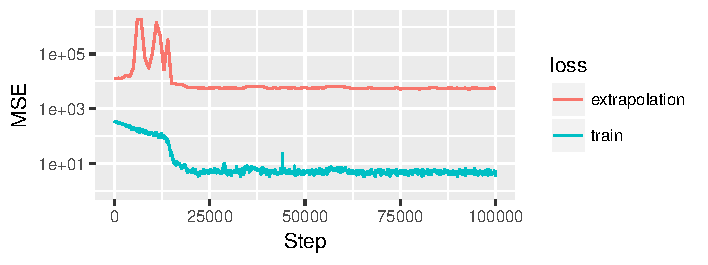
\includegraphics[]{./graphics/nac-mul-normal-learning}
	\caption{Train error, and extrapolation error. In the extrapolation dataset $x_i \sim \mathrm{Uniform}[1, 6]$ is used.}
\end{figure}

\section{Known Issues}

To better describe the known issues we have found, the network is first re-expressed using scalar notation:

\begin{equation}
\begin{aligned}
z_{h_1} &= \sum_{h_0=1}^{H_0} w_{h_1, h_0} z_{h_0} \\
z_{h_2} &= \exp\left(\sum_{h_1=1}^{H_1} w_{h_2, h_1} \log(|z_{h_1}| + \epsilon) \right) \\
\mathcal{L} &= \sum_{h_2=1}^{H_2} (z_{h_2} - t_{h_2})^2
\end{aligned}
\end{equation}


\subsection{Gradient of $\tanh(\hat{\mathbf{W}}) \odot \sigma(\hat{\mathbf{M}})$}

The problem with the soft constrained weight matrix, is best seen with its gradient:

\begin{equation}
\begin{aligned}
\frac{\partial \mathcal{L}}{\partial \hat{w}_{h_{\ell-1},h_\ell}} &= \frac{\partial \mathcal{L}}{\partial w_{h_{\ell-1},h_\ell}} (1 - \tanh^2(\hat{w}_{h_{\ell-1},h_\ell})) \sigma(\hat{m}_{h_{\ell-1},h_\ell}) \\
\frac{\partial \mathcal{L}}{\partial \hat{m}_{h_{\ell-1},h_\ell}} &= \frac{\partial \mathcal{L}}{\partial w_{h_{\ell-1},h_\ell}} \tanh(\hat{w}_{h_{\ell-1},h_\ell}) \sigma(\hat{m}_{h_{\ell-1},h_\ell}) (1 - \sigma(\hat{m}_{h_{\ell-1},h_\ell}))
\end{aligned}
\end{equation}

As expected the gradient becomes very small at its boundaries. This in itself hurts the networks ability to explore once the weight have reached one of its boundaries. However, more problematic is that $\tanh(\hat{w}_{h_{\ell-1},h_\ell})$ for an initialization with $E[\hat{w}_{h_{\ell-1},h_\ell}] = 0$, causes to the gradient $\frac{\partial \mathcal{L}}{\partial \hat{m}_{h_{\ell-1},h_\ell}}$ to have zero as its expectation.

Finally, we have observed that while this weight matrix construction does have the desired constraints, there is nothing that prevents it from attaining values between $-1$ and $0$, or $1$ and $0$. This is particularly observed for the problem of adding the sum of two subsets, where an optimal solution can be found. But the optimal solution often uses these ``mixed'' weights.

Instead of using $\tanh(\hat{\mathbf{W}}) \odot \sigma(\hat{\mathbf{M}})$ to constrain the weight matrix, we have observed that a purely linear unit with a regularizer works much better.

The regularizer is:
\begin{equation}
\mathcal{R_\ell} = \sum_{h_{\ell-1}=1}^{H_{\ell-1}} \sum_{h_{\ell}=1}^{H_{\ell}} \hat{w}_{h_{\ell-1},h_\ell}^2 (1 - |w_{h_{\ell-1},h_\ell}|)^2 
\end{equation}

\subsection{Logarithm for small hidden values}

The logarithm $\log(|z_{h_1}| + \epsilon)$ naturally have its issues, when $z_{h_1}$ is near zero. This is in fact quite likely as $E[z_{h_1}] = 0$ when an initialization with $E[w_{h_{\ell-1},h_\ell}] = 0$ is used.

A solution that we propose, is to not support $z_{h_1} < 1$. This allows us to use a safe-log instead:   

\begin{equation}
z_{h_2} = \exp\left(\sum_{h_1=1}^{H_1} w_{h_2, h_1} \log(|z_{h_1} - 1| + 1) \right)
\end{equation}

The issue can easily be visualized by considering the following simplification of our model. $x$ and $t$ are set to static values, and $\mathbf{W_1}$ and $\mathbf{W_2}$ are reduced to just two scalar parameters.

\begin{equation*}
\begin{aligned}
\mathbf{x} &= [1, 1, 2, 2],& t &= 12 \\
\mathbf{W_1} &= \begin{bmatrix}
w_1 & w_1 & 0 & 0 \\
w_1 & w_1 & w_1 & w_1
\end{bmatrix},& 
\mathbf{W_2} &= \begin{bmatrix}
w_2 & w_2
\end{bmatrix}
\end{aligned}
\end{equation*}

\begin{figure}[H]
	\centering
\begin{subfigure}{.5\textwidth}
  \centering
  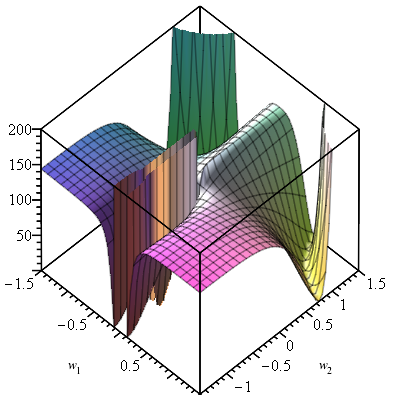
\includegraphics[width=\linewidth]{./graphics/nac-mul-normal-loss.png}
  \caption{Using $\log(|\mathbf{z_1}| + \epsilon)$}
\end{subfigure}%
\begin{subfigure}{.5\textwidth}
  \centering
  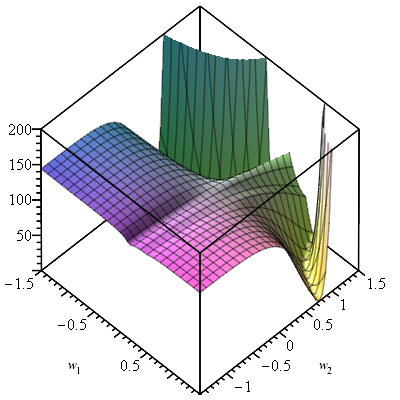
\includegraphics[width=\linewidth]{./graphics/nac-mul-safe-loss.png}
  \caption{Using $\log(|\mathbf{z_1} - 1| + 1)$}
\end{subfigure}
	\caption{Loss curvature.}
\end{figure}

Experiments with using $\log(\max(0, \mathbf{z_1} - 1) + 1)$ have also been performed. In some cases this provide even better results, but the challenge is that there is no gradient for all input values less than one. However, even when this is not an issue, the problem still doesn't converge.

\subsection{Gradient of Multiplicative NAC}

The weight gradient for the multiplicative NAC is:
\begin{equation}
\frac{\partial \mathcal{L}}{\partial w_{h_2, h_1}} = \frac{\partial \mathcal{L}}{\partial z_{h_2}} \frac{\partial z_{h_2}}{\partial w_{h_2, h_1}} = \frac{\partial \mathcal{L}}{\partial z_{h_2}} z_{h_2} \log(|z_{h_1}| + \epsilon)
\end{equation}

The backpropagation value is:
\begin{equation}
\frac{\partial \mathcal{L}}{\partial z_{h_1}} = \sum_{h_2 = 1}^{H_2} \frac{\partial \mathcal{L}}{\partial z_{h_2}} \frac{\partial z_{h_2}}{\partial z_{h_1}} = \sum_{h_2 = 1}^{H_2} \frac{\partial \mathcal{L}}{\partial z_{h_2}} z_{h_2} w_{h_2, h_1} \frac{\mathrm{abs}'(z_{h_1})}{|z_{h_1}| + \epsilon}
\end{equation}

Thus the full gradients for the entire network are:
\begin{equation*}
\begin{aligned}
\frac{\partial \mathcal{L}}{\partial w_{h_1, h_0}} &= \frac{\partial \mathcal{L}}{\partial z_{h_1}} z_{h_0} &&= 2 \cdot \frac{\mathrm{abs}'(z_{h_1})}{|z_{h_1}| + \epsilon} z_{h_0} \sum_{h_2 = 1}^{H_2} (z_{h_2} - t_{h_2}) z_{h_2} w_{h_2, h_1} \\
\frac{\partial \mathcal{L}}{\partial w_{h_2, h_1}} &= \frac{\partial \mathcal{L}}{\partial z_{h_2}} z_{h_2} \log(|z_{h_1}| + \epsilon) &&= 2 \cdot (z_{h_2} - t_{h_2}) z_{h_2} \log(|z_{h_1}| + \epsilon)
\end{aligned}
\end{equation*}

This reveals some issues. Given that a desired initialization property typically is $E[z_{h_1}] = 0, E[z_{h_2}] = 0$, the gradients should explode for a typical initialization.

Also, although the issue of $E[z_{h_1}] = 0$ issue solved if the ``safe-log'' variant is used. The $z_{h_2}$ still creates the possibility of an exploding gradient. Besides this, its shared existence in all gradients means that there is a large interdependency. This appears to cause parameter oscillation, even for small learning rates.

\subsection{No ideal initialization}

Based on the work on Glorot et. al. and He et. al, the idea initialization has $E[z_{h_\ell}] = 0$ and $Var[z_{h_\ell}] = Var(z_{h_0})$. Likewise for the backpropagation as well.

It is possible to show, using some Taylor approximation and assumptions of uncorrelated stochastic variables that we have:

\begin{equation}
\begin{aligned}
E[z_{h_1}] &= 0 \\
Var[z_{h_1}] &= H_1 Var\left[W_{h_0, h_1}\right] Var[z_{h_0}]\\
E[z_{h_2}] &\approx\left(1 + \frac{1}{2} Var[W_{h_2, h_1}] \log(|E[z_{h_1}]| + \epsilon)^2\right)^{H_1} \\
Var[z_{h_2}] &\approx \left(1 + 2 \cdot Var[W_{h_2, h_1}] \log(|E[z_{h_1}]| + \epsilon)^2\right)^{H_1} \\
&- \left(1 + \frac{1}{2} \cdot Var[W_{h_2, h_1}] \log(|E[z_{h_1}]| + \epsilon)^2\right)^{2\cdot H_1}
\end{aligned}
\end{equation}

\begin{equation}
\begin{aligned}
E\left[\frac{\partial \mathcal{L}}{\partial z_{h_1}}\right] &= 0 \\
Var\left[\frac{\partial \mathcal{L}}{\partial z_{h_1}}\right] &\approx Var\left[\frac{\partial \mathcal{L}}{\partial z_{h_2}}\right] H_2 \left(1 + 2 \cdot Var[W_{h_2, h_1}] \log(|E[z_{h_1}]| + \epsilon)^2\right)^{H_1} \\
&\cdot Var[W_{h_2, h_1}] \left(\frac{1}{\left(|E[z_{h_1}]| + \epsilon\right)^2} + \frac{3}{\left(|E[z_{h_1}]| + \epsilon\right)^4} Var[z_{h_1}]\right)
\end{aligned}
\end{equation}
s
As seen from these approximations, $E[z_{h_2}] = 0$ is not possible. Likewise maintaining constant variance is also not possible. This might not be a problem when considering only two layers, but for more complex networks this will likely create an exploding gradient issue.

\section{Next step}

We would like to understand more deeply the problems of convergence of this problem. While we have uncovered some issues, it still does not seam justifiable that such as simple network can't converge.

Even with our suggested improvements, it is still not possible to optimize towards a valid solution. 

\section{Additional Information}

In the context of the NALU, which Google DeepMind clams work. There are a few things to understand, in why it could converge given a very lucky seed.

\begin{itemize}
\item The gate itself, is problematic because the initial expectation and gradient of the multiplication and addition operators behaves significantly differently. A network will thus almost always converge to addition, as this have a higher and more stable gradient. Thus the addition operator becomes the best estimator, first. Once an operator have been learned, the network doesn't explore other solutions as it is stuck in a local minima.
\item They don't include the a bias term in the gating mechanism, because this artificially increases exploration.
\item They share the weight matrix between addition and multiplication, because for positive inputs, addition and multiplication are correlated. Thus if the network is initially converging to an addition operator (it almost always will due to expectation differences), the multiplication operator will still converge towards something meaningful. For a very lucky seed, the multiplication operator could become so good that it becomes a better estimator than the addition operator. Thus the gate will switch to multiplication.
\end{itemize}

We have contacted the authors about a month ago, just to understand in more detail how they setup the problem. Such as, how is the input vector distributed. However, their response have been close to non-existing and the few answers we have gotten have been extremely wage, considering the simplicity of the questions.

\section{References}
\printbibliography[heading=none]

\end{document}